\chapter{Grupo Empresarial CIMEX: gestión comercial}\label{chapter:proposal}

En toda empresa para mantener un rendimiento ascendente es de vital importancia que los directivos y analistas presenten un acceso cómodo y fiable a información útil y valiosa referente al desempeño del negocio. La base de este tipo de sistema de información son los datos recuperados, conciliados, almacenados, posteriormente analizados y convertidos en conocimiento, todo lo cual debe contribuir de forma satisfactoria a la toma de decisiones en la empresa.\\

El Grupo Empresarial CIMEX es una de las principales entidades que presenta el país dedicadas al comercio y la exportación, es considerada entre las primeras organizaciones en utilizar soluciones computacionales con el fin de favorecer la toma de decisiones. En el presente capitulo se explica brevemente el funcionamiento de el negocio, las aplicaciones que se han implementado hasta el momento para la toma de decisiones, esencialmente en términos de la información comercial, así como la descripción del escenario actual que propicia el desarrollo de la presente investigación en función de lograr una nueva aproximación de solución de inteligencia de negocios.


\section*{Grupo Empresarial CIMEX}\label{CIMEX}
\addcontentsline{toc}{section}{Grupo Empresarial CIMEX}
La Corporación de Exportación e Importación (CIMEX) es una sociedad de capital estatal cubano compuesta por numerosas entidades cuyo principal objetivo es la adquisición y la comercialización de productos y servicios. Esta maneja un amplio conjunto de líneas de negocio que comprende desde la comercialización de forma minorista y mayorista hasta otros relacionados con la importación y la exportación de mercancías y el transporte marítimo, así como los servicios de gastronomía, tecnológicos y de aduana.\\

La corporación se encuentra estructurada en vicepresidencias y direcciones, sucursales territoriales, sociedades afiliadas y divisiones especializadas. Una de las divisiones especializadas es la División DATACIMEX, encargada de poner a disposición de los usuarios de CIMEX una amplia gama de aplicaciones computacionales que facilitan sus actividades. Hace más de diez años en DATACIMEX se comenzó a trabajar en la transformación de los datos primarios en función de la toma de decisiones.\\

El grupo de Inteligencia de Negocios, perteneciente a esta División, ha desarrollado desde el año 2008 un portal web para el apoyo a la toma de decisiones, denominado Sistema de Administración de Negocios (SAN). En SAN se muestran reportes estáticos sobre diferentes procesos de negocio que se interrelacionan en la organización, brindando a los directivos un conjunto de aplicaciones que abarcan desde la etapa de planificación y ejecución de cada uno de los procesos hasta la evaluación de comportamientos mediante indicadores, cuadros de mando y emisión automática de boletines.



\section*{Gestión Comercial relacionada con las Estadísticas Minoristas}\label{gestion_comercial}
\addcontentsline{toc}{section}{Gestión Comercial relacionada con las Estadísticas Minoristas}
Una de las actividades fundamentales de la corporación es el comercio minorista. Las entidades pertenecientes a este comercio son también conocidas como entidades. Esta red de establecimientos  minoristas está conformada por: Las tiendas Panamericanas, los Servicentros Cupet y Oro Negro, las cafeterías El Rápido, los videocentros, las tiendas fotográficas Photoservice, los centros comerciales y las pequeñas tiendas en los barrios, denominadas puntos de venta.\\

La red está organizada de forma jerárquica teniendo en su nivel más alto a las Sucursales, las cuales se dividen en Centros Contables o Complejos, los que a su vez se subdividen en Establecimientos Independientes, formados por Establecimientos Dependientes (Figura 2.1).


\begin{figure}[ht]
  \begin{center}
    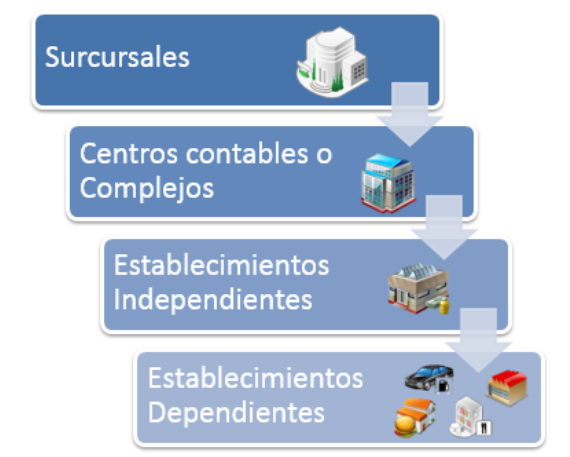
\includegraphics[scale=0.4]{Graphics/figura2_1.png}
    \caption{Red minorista de CIMEX.}
    \label{fig:red minorista}
  \end{center}
\end{figure}

%%
% IMAGEN
%%

La actividad comercial de las tiendas minoristas genera diariamente gran cantidad de información la cual es necesaria mantener actualizada y administrada de forma fiable para lograr un mejor desempeño para las analistas y directivos de la corporación y también otras entidades pertenecientes al país como son la Oficina Nacional de Estadísticas e Información (ONEI) y el Ministerio de Comercio Interior (MINCIN). Desde la perspectiva comercial se realizan varias operaciones que provocan movimientos de entrada y salida en el inventario relacionadas con los conceptos compra y venta de mercancías, transferencias y ajustes. Es necesario mantener un seguimiento periódico del comportamiento de estas operaciones, pues con un análisis certero y previsor se evitan posibles desabastecimientos o sobre-inventarios y es posible aumentar el nivel de las ventas y la satisfacción del cliente. Estos comportamientos se analizan a partir de un conjunto de indicadores comerciales.


\section*{Conceptos Comerciales}\label{concepto_comercial}
\addcontentsline{toc}{section}{Conceptos Comerciales}
En un establecimiento de la red minorista de CIMEX se realizan varias actividades comerciales como venta de mercancías, servicios fotográficos, venta de combustible y servicios de gastronomía. Además existen diferentes áreas o localidades, entre las que se encuentran almacén, merma y venta. Para mantener correctos los niveles de inventario en las tiendas y en los almacenes centrales es necesario efectuar el seguimiento sistemático del comportamiento del negocio en relación con las ventas.\\

Los conceptos en el ámbito comercial manejados por CIMEX son:

\begin{itemize}
\item \textbf{Compras:} Representan el acto mediante el cual CIMEX, como sujeto económico, entra en posesión de un bien o servicio mediante el pago del precio a un proveedor. (La Gran Enciclopedia de Economía, 2009) 
\item \textbf{Ventas:} Representan las entregas a clientes de productos terminados, trabajos efectuados, servicios prestados y mercancías. (Grupo Empresarial CIMEX, 1999) 
\item \textbf{Inventario:} Es el conjunto de mercancías o artículos acumulados en el almacén en espera de ser vendidos o utilizados en el proceso productivo. (La Gran Enciclopedia de Economía, 2009) Es decir, representa la existencia física de todos los productos en un establecimiento. 
\item \textbf{Transferencias:} Responden a los movimientos de mercancías entre establecimientos o entre localidades de un mismo establecimiento, por ejemplo, del almacén al área de ventas. Un movimiento de mercancía se registra en los sistemas de control como una transferencia de salida en el origen y una transferencia de entrada en el destino.
\item \textbf{Ajustes:} Engloban todas las operaciones que se realizan en el inventario de un establecimiento para reflejar los niveles de existencia reales. Por ejemplo, los faltantes y sobrantes en un establecimiento, que se detectan en el conteo físico, deben ser ajustados en el sistema de control, sea o no computacional, para que quede reflejado en el inventario real del establecimiento. Otros motivos para realizar ajustes son los errores que se cometen al registrar una operación de venta o transferencia y la afectación del inventario por rotura o deterioro de los productos.
\item \textbf{Vales:} Responden a la entrada o la salida del inventario de mercancías mediante otro concepto que no sea Compra o Venta. El vale de entrada representa la recepción de mercancía que no fue comprada a un proveedor, por ejemplo, una donación. El vale de entrega representa la salida del inventario de mercancía que no fue vendida sino que se traslada del establecimiento a otras entidades que no pertenecen a CIMEX, previo acuerdo entre las partes. 
\end{itemize}  


\section*{Soluciones Precedentes}\label{sol_presed}
\addcontentsline{toc}{section}{Soluciones Precedentes}
El análisis de las Estadísticas Minoristas en la corporación ha pasado en el decursar de los años por diferentes soluciones para la concepción y análisis de la información mediante los estadistas. Se ha priorizado tanto la automatización de sus principales operaciones empresariales como la evolución necesaria de acuerdo con el desarrollo científico, tecnológico y profesional en sus entidades. No solo se han dado respuestas oportunas y pertinentes al procesamiento de los datos operacionales sino también se ha trabajado con el propósito de facilitar los procesos de dirección con herramientas y ambientes computacionales propios, que han sentado las bases para el desarrollo de la presente investigación.\\

Con anterioridad la empresa contaba con diferentes sistemas computacionales encargados de la recolección de la informacion ERP (Enterprise Resource Planning) los cuales eran: Silver, Sentai-Trax y Sentai-Viper. Por razones ajenas a la investigación de la presente tesis en la actualidad se cuenta con un único ERP conocido como Sentai el cual presenta la información que será utilizada por los analistas y directivos.\\

En el año 2000 se desarrolló en CIMEX una solución implementada en el lenguaje de programación Visual Foxpro 5.0, que brindaba funcionalidades para el análisis de los indicadores comerciales minoristas. Consistía en una aplicación de escritorio instalada en cada una de las sucursales y una versión central en la dirección de CIMEX (Figura 2.3). Esta primera aproximación logró resolver las necesidades básicas de información, entre ellas la presentación de ciertos indicadores comerciales como la utilidad de la venta de un producto en un mes o la acumulada en el año actual. Los principales resultados que produjo este sistema fueron: 

\begin{itemize}
\item Ubicó a CIMEX entre las primeras organizaciones cubanas en diseñar una solución computacional en términos de la toma de decisiones. 
\item Constituyó la primera solución que unificaba los datos disgregados en los diferentes sistemas operacionales, permitiendo el seguimiento de los indicadores comerciales.
\item Logró brindar un conjunto de funcionalidades básicas para el análisis y la toma de decisiones, tales como visualizar reportes parametrizados de los principales indicadores comerciales.
\item El lenguaje de programación Visual Foxpro 5.0 se convirtió en obsoleto, lo que dificultó la realización de actualizaciones.
\item La interfaz visual no era intuitiva.  
\item En una misma consulta no era posible realizar comparaciones entre diferentes años. 
\item Los mecanismos de sincronización entre las diferentes instancias de la aplicación no eran suficientes y se limitaba la actualización de los datos.
\end{itemize}

Posteriormente, en el período comprendido entre los años 2003 y 2006 se desarrolló un sistema centrado en la actividad comercial que se alimentaba de un data warehouse. Esta solución marcó un nuevo comienzo en el desarrollo de soluciones de inteligencia de negocios en CIMEX, ya que por primera vez se utilizó un repositorio de datos basado en el modelo dimensional. Las cuestiones fundamentales que en aquellos momentos llevaron a la elección de este modelo fueron la necesidad de garantizar la homogenización de los datos para el análisis, el mantenimiento de los datos históricos, la ganancia en eficiencia y el requisito de brindar la posibilidad de navegar de forma sencilla y organizada a través de la información con cierto dinamismo. \\

En el DW estaban representados los sujetos del negocio en cubos disímiles, con el objetivo de poseer la información desglosada, facilitándose el análisis y la toma de decisiones. La solución brindaba al usuario la posibilidad de definir con cierto dinamismo cómo deseaba visualizar la información, así como las condiciones de búsqueda. Estas posibilidades permiten afirmar que se logró un paso de avance con respecto a los reportes existentes en la solución anterior. \\

A pesar de las ventajas de esta aproximación, su puesta en práctica demostró que en CIMEX no estaban creadas las condiciones para su explotación, debido fundamentalmente a las razones que se enumeran a continuación: 

\begin{itemize}
\item El proceso de integración de los datos no garantizaba la actualización eficiente del DW, por lo que no era posible satisfacer ciertos requerimientos informacionales.
\item No siempre las salidas de los sistemas operacionales requeridas para la actualización del DW estaban disponibles oportunamente. 
\item Los usuarios demandaban reportes más específicos que le resolvieran necesidades cruciales de información que no estaban satisfechas aún, tales como alertas de reabastecimiento.
\item No había suficiente madurez en el uso de las herramientas computacionales para aprovechar las bondades de navegación y construcción dinámica de sus propios reportes, aun cuando se realizaron intentos por inculcar la nueva filosofía de trabajo a los analistas y los ejecutivos
\end{itemize}

Posteriormente en el 2008 se concibe una solución la cual encararía los problemas presentes hasta ese momento, consistiendo la misma en la creación de un almacén de datos operacionales como repositorio de datos conciliados, que posteriormente se derivan en otra base de datos propia de la aplicación. Esta nueva solución presentaría muchos puntos positivos como serian:

\begin{itemize}
\item Los datos se encuentran centralizados, consolidados y resumidos de forma conveniente.
\item Se posibilita la generación dinámica de informes a partir de los datos informacionales dentro de algunas de las plantillas predefinidas en la aplicación.
\item Los resultados finales se visualizan con SQL Server Reporting Services, que permite la distribución de reportes en distintos formatos (hojas de Excel, documentos PDF, documentos Word, entre otros).
\item La interfaz de usuario es más amigable y se enriquece la presentación final de la información.
\end{itemize}


Pero a su vez esta está quedando obsoleta con respecto a las nuevas necesidades presentes en la empresa mostrándose inconvenientes con respecto a la mudanza de la corporación al trabajo con software de código abierto.


